\chapter{Conformal Mapping, Laplace's Equation, and Open-String Scattering}

These notes follow Leonard Susskind's lecture in the order in which the argument is actually built. The lecture record curated by LazyingArt LLC and Video2Book is especially helpful here because the mathematics is carried both by the spoken motivation and by the blackboard layout. We begin not with string scattering itself, but with two-dimensional electrostatics, because that is where conformal mapping first becomes physically natural rather than formally decorative.

\section{Electrostatics As The First Model For Conformal Mapping}

Susskind wants conformal mapping to feel earned. So he begins with a concrete question: if electric flux is forced to remain in a plane, what becomes of Coulomb's law? In two dimensions the force is weaker than in three-dimensional electrostatics,
\begin{equation}
F(r)\propto \frac{1}{r},
\end{equation}
and the corresponding potential energy is logarithmic,
\begin{equation}
V(r)\propto \log r.
\end{equation}
That already tells us that planar electrostatics is not just a trivial reduction of the three-dimensional story. It is a different mathematics.

The simpler object is not the electric field itself but the scalar potential \(\phi\). Following the lecture's sign convention, we write
\begin{align}
\mathbf E &= \nabla \phi, \\
\nabla\cdot \mathbf E &= \rho.
\end{align}
Combining them gives the Poisson equation
\begin{equation}
\nabla^2\phi=\rho.
\end{equation}
In a literal two-dimensional world with coordinates \(x\) and \(y\), the Laplacian is
\begin{equation}
\nabla^2\phi=\frac{\partial^2\phi}{\partial x^2}+\frac{\partial^2\phi}{\partial y^2}.
\end{equation}
Away from charges the right-hand side vanishes, so one has the source-free Laplace equation
\begin{equation}
\frac{\partial^2\phi}{\partial x^2}+\frac{\partial^2\phi}{\partial y^2}=0.
\end{equation}

\begin{figure}[h]
\centering

\includegraphics[width=0.62\textwidth]{lecture_08_figure_02.png}
\caption{Electrostatic equations and the two-dimensional Laplacian.}
\end{figure}

This is the first important point of contact with conformal mapping. The two-dimensional Laplace equation is unchanged by conformal coordinate transformations, and that means a solution on one domain can be carried to a solution on another. This is why conformal maps matter in electrostatics, fluid flow, and eventually on the string worldsheet.

\subsection{Question \& Answer}

\paragraph{Question.} Why are these not wave equations?

\paragraph{Answer.} Because the equation on the board is elliptic, not hyperbolic. In empty space it reads
\[
\partial_x^2\phi+\partial_y^2\phi=0,
\]
with no time derivative at all, and with a plus sign between the spatial second derivatives. To describe waves one must introduce time dependence as an independent variable. Electrostatics is static precisely because nothing is moving.

There is also a brief aside in the lecture about curl in two dimensions. If
\[
\mathbf E=(E_x,E_y),
\]
then the curl has only one component,
\begin{equation}
\operatorname{curl}_{2d}\mathbf E=\frac{\partial E_x}{\partial y}-\frac{\partial E_y}{\partial x}.
\end{equation}
It is best thought of here not as a full vector but as the one scalar quantity that survives in two dimensions.

\section{Complex Coordinates And The Problem Of A Unique Derivative}

Now the lecture pivots from electrostatics to the plane itself. We write the original plane in complex notation as
\begin{equation}
z=x+iy,
\end{equation}
and the image plane as
\begin{equation}
w=u+iv.
\end{equation}
A mapping of the plane to itself is then a complex function \(w(z)\), or equivalently a coordinate transformation from \((x,y)\) to \((u,v)\). The lecture assumes the mapping is one-to-one, so each point in one plane corresponds to a unique point in the other.

The central new question is not continuity. It is differentiability. For a real variable there are only two directions of approach, but for a complex variable there are infinitely many. So the natural definition
\begin{equation}
\frac{dw}{dz}=\lim_{\Delta z\to 0}\frac{\Delta w}{\Delta z}
\end{equation}
is only meaningful if the answer is independent of the direction from which \(\Delta z\) approaches zero.

\subsection{Question \& Answer}

\paragraph{Question.} What condition makes \(dw/dz\) well defined in the complex plane?

\paragraph{Answer.} The limit must not depend on direction. Susskind compares approach along the \(x\)-axis with approach along the \(y\)-axis. If the two agree, one gets the right condition; and in fact that condition is also sufficient.

Along the \(x\)-axis one has \(dy=0\), so
\begin{equation}
\frac{dw}{dz}=\frac{\partial u}{\partial x}+i\frac{\partial v}{\partial x}.
\end{equation}
Along the \(y\)-axis one has \(dx=0\), so
\begin{equation}
\frac{dw}{dz}=\frac{1}{i}\frac{\partial u}{\partial y}+\frac{\partial v}{\partial y}
=\frac{\partial v}{\partial y}-i\frac{\partial u}{\partial y}.
\end{equation}
If these are to be the same derivative, their real and imaginary parts must agree.

\section{Cauchy-Riemann Equations And Harmonic Functions}

Equating the two directional expressions for \(dw/dz\) gives the Cauchy-Riemann equations:
\begin{align}
\frac{\partial u}{\partial x} &= \frac{\partial v}{\partial y}, \\
\frac{\partial u}{\partial y} &= -\,\frac{\partial v}{\partial x}.
\end{align}
This is the condition for the complex derivative to exist in a unique way. A function that satisfies it is analytic at the point in question; if it is analytic everywhere, the lecture calls it entire.

The point is not merely that these equations are pretty. The point is that they return us straight to Laplace's equation. Differentiate the first equation with respect to \(x\):
\begin{equation}
\frac{\partial^2 u}{\partial x^2}=\frac{\partial^2 v}{\partial x\,\partial y}.
\end{equation}
Differentiate the second with respect to \(y\):
\begin{equation}
\frac{\partial^2 u}{\partial y^2}=-\,\frac{\partial^2 v}{\partial x\,\partial y}.
\end{equation}
Add them, and the mixed partial derivatives cancel:
\begin{equation}
\frac{\partial^2 u}{\partial x^2}+\frac{\partial^2 u}{\partial y^2}=0.
\end{equation}
The same trick, with \(x\) and \(y\) interchanged at the right places, gives
\begin{equation}
\frac{\partial^2 v}{\partial x^2}+\frac{\partial^2 v}{\partial y^2}=0.
\end{equation}

So an analytic function \(w=u+iv\) contains two real harmonic functions. That is the bridge back to electrostatics: analytic maps are built out of Laplace solutions.

There is also a pleasant vector interpretation. If we package the two real functions as the vector field \((u,-v)\), then the Cauchy-Riemann equations become
\begin{align}
\frac{\partial u}{\partial x}-\frac{\partial v}{\partial y} &= 0, \\
\frac{\partial u}{\partial y}+\frac{\partial v}{\partial x} &= 0.
\end{align}
The first is vanishing divergence, and the second is the two-dimensional curl condition.

\section{Why Analytic Functions Are Conformal}

This is the payoff promised from the start. We do not simply assert that analytic maps are conformal. We prove it in the language of small intervals and phases.

A small complex displacement can be written in polar form as
\begin{equation}
\delta z=\rho e^{i\theta}, \qquad \Delta z=\rho' e^{i\theta'}.
\end{equation}
Then the ratio is
\begin{equation}
\frac{\delta z}{\Delta z}=\frac{\rho}{\rho'}e^{i(\theta-\theta')}.
\end{equation}
The important fact is that the phase of a ratio is the difference of the phases. In other words, the argument of the ratio is the angle between the two displacements.

Now take two small intervals \(\delta z\) and \(\Delta z\) meeting at one point in the \(z\)-plane, and let them map to \(\delta w\) and \(\Delta w\) in the \(w\)-plane. If \(w(z)\) is analytic, then the derivative exists and is direction-independent, so
\begin{equation}
\frac{\delta w}{\delta z}=\frac{\Delta w}{\Delta z}.
\end{equation}
Rearranging,
\begin{equation}
\frac{\Delta z}{\delta z}=\frac{\Delta w}{\delta w}.
\end{equation}
But the phase of the left-hand side is precisely the angle between the two intervals in the \(z\)-plane, and the phase of the right-hand side is the angle between their images in the \(w\)-plane. Therefore the two angles are equal. That is exactly the defining property of a conformal map.

\begin{figure}[h]
\centering
\begin{tikzpicture}[scale=1.0]
\draw[->] (-1.4,0) -- (1.6,0);
\draw[->] (0,-1.2) -- (0,1.6);
\node at (0,-1.5) {$z$-plane};
\fill (0,0) circle (0.04);
\draw[->] (0,0) -- (1.15,0.42);
\draw[->] (0,0) -- (0.48,1.12);
\node at (1.18,0.65) {$\delta z$};
\node at (0.72,1.28) {$\Delta z$};
\draw (0.48,0.17) arc (20:67:0.50);

\begin{scope}[xshift=5.2cm]
\draw[->] (-1.4,0) -- (1.6,0);
\draw[->] (0,-1.2) -- (0,1.6);
\node at (0,-1.5) {$w$-plane};
\fill (0,0) circle (0.04);
\draw[->] (0,0) -- (1.18,0.50);
\draw[->] (0,0) -- (0.54,1.18);
\node at (1.22,0.74) {$\delta w$};
\node at (0.78,1.34) {$\Delta w$};
\draw (0.50,0.21) arc (23:66:0.54);
\end{scope}
\end{tikzpicture}
\caption{Two infinitesimal intervals in the \(z\)-plane and their images in the \(w\)-plane. Analyticity preserves the angle between them.}
\end{figure}

\subsection{Question \& Answer}

\paragraph{Question.} Why does analyticity imply angle preservation?

\paragraph{Answer.} Because analyticity says that the same derivative relates every infinitesimal interval through the point. When two intervals are compared by taking a ratio, the derivative cancels out, and what remains is the ratio of the intervals themselves. The phase of that ratio is the angle between them. So the angle in the \(z\)-plane and the angle in the \(w\)-plane must be the same.

At this point the lecture makes the identification explicit: analytic coordinate changes are not merely examples of conformal maps. They are the conformal coordinate changes relevant for the equations of motion on the string worldsheet.

\section{Examples And Global Maps}

\paragraph{Worked example: \(W=z^2\).} The blackboard first takes the very simple map \(W=z^2\). Writing \(z=x+iy\),
\begin{align}
W &= z^2, \\
(x+iy)^2 &= x^2-y^2+2ixy=u+iv.
\end{align}
So
\begin{equation}
u=x^2-y^2, \qquad v=2xy.
\end{equation}

\begin{figure}[h]
\centering

\includegraphics[width=0.72\textwidth]{lecture_08_figure_03.png}
\caption{The map \(W=z^2\) and the identification of \(u\) and \(v\).}
\end{figure}

Now check the Laplace equations directly:
\begin{align}
\frac{\partial^2 u}{\partial x^2} &= 2, &
\frac{\partial^2 u}{\partial y^2} &= -2,
\end{align}
so
\begin{equation}
\frac{\partial^2 u}{\partial x^2}+\frac{\partial^2 u}{\partial y^2}=0.
\end{equation}
For \(v=2xy\),
\begin{equation}
\frac{\partial^2 v}{\partial x^2}=0, \qquad \frac{\partial^2 v}{\partial y^2}=0,
\end{equation}
and therefore \(v\) is harmonic too. This is exactly the sort of check Susskind wants: one moves back and forth between complex algebra and the real Laplace equation.

A useful non-example is the complex conjugate,
\begin{equation}
w=\bar z=x-iy.
\end{equation}
Then
\begin{equation}
u=x, \qquad v=-y,
\end{equation}
so
\begin{equation}
\frac{\partial u}{\partial x}=1, \qquad \frac{\partial v}{\partial y}=-1.
\end{equation}
The first Cauchy-Riemann equation already fails, and therefore \(w=\bar z\) is not analytic. The minus sign ruins it.

A richer analytic example is
\begin{equation}
w=e^z=e^{x+iy}=e^x(\cos y+i\sin y),
\end{equation}
so
\begin{equation}
u=e^x\cos y, \qquad v=e^x\sin y.
\end{equation}
Then
\begin{align}
\frac{\partial u}{\partial x} &= e^x\cos y = \frac{\partial v}{\partial y}, \\
\frac{\partial u}{\partial y} &= -e^x\sin y = -\,\frac{\partial v}{\partial x},
\end{align}
and the Cauchy-Riemann equations hold exactly.

The lecture then turns from local examples to global geometry. For the logarithm map we write
\begin{equation}
z=re^{i\theta},
\end{equation}
and therefore
\begin{equation}
w=\log z=\log r+i\theta.
\end{equation}
If we restrict to the right half-plane, then
\begin{equation}
-\frac{\pi}{2}\leq \theta \leq \frac{\pi}{2},
\end{equation}
so the image is a strip
\begin{equation}
-\frac{\pi}{2}\leq \Im w \leq \frac{\pi}{2}.
\end{equation}
Lines of constant angle become horizontal lines, and circles of constant radius become vertical lines. Translation along the strip corresponds to dilation in the half-plane.

\begin{figure}[h]
\centering
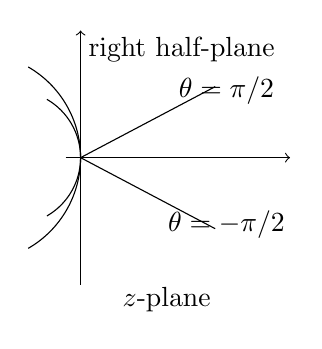
\begin{tikzpicture}[scale=0.95]
\draw[->] (-0.2,0) -- (2.8,0);
\draw[->] (0,-1.7) -- (0,1.7);
\draw (0,-1.45) -- (0,1.45);
\draw (0,0) -- (2.1,0);
\draw (0,0) -- (1.8,0.95);
\draw (0,0) -- (1.8,-0.95);
\draw (0,0) arc (0:60:0.9);
\draw (0,0) arc (0:-60:0.9);
\draw (0,0) arc (0:60:1.4);
\draw (0,0) arc (0:-60:1.4);
\node at (1.35,1.45) {right half-plane};
\node at (1.15,-1.9) {$z$-plane};
\node at (1.95,0.90) {$\theta=\pi/2$};
\node at (1.95,-0.90) {$\theta=-\pi/2$};
\end{tikzpicture}
\hspace{0.8cm}
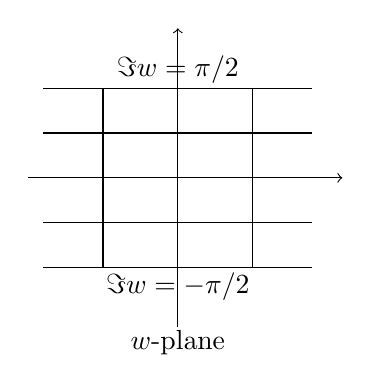
\begin{tikzpicture}[scale=0.95]
\draw[->] (-2.0,0) -- (2.2,0);
\draw[->] (0,-2.0) -- (0,2.0);
\draw (-1.8,1.2) -- (1.8,1.2);
\draw (-1.8,-1.2) -- (1.8,-1.2);
\draw (-1.0,-1.2) -- (-1.0,1.2);
\draw (0,-1.2) -- (0,1.2);
\draw (1.0,-1.2) -- (1.0,1.2);
\draw (-1.8,0.6) -- (1.8,0.6);
\draw (-1.8,0) -- (1.8,0);
\draw (-1.8,-0.6) -- (1.8,-0.6);
\node at (0,1.45) {$\Im w=\pi/2$};
\node at (0,-1.45) {$\Im w=-\pi/2$};
\node at (0,-2.2) {$w$-plane};
\end{tikzpicture}
\caption{The logarithm map sends the right half-plane to a strip.}
\end{figure}

If instead we map the whole plane, then the angular variable is periodic modulo \(2\pi\). The strip therefore has its top identified with its bottom, and the image is an infinite cylinder. This is already suggestive physically: half-plane and strip are natural for open strings, while the full plane and cylinder are natural for closed strings.

For the map from half-plane to disk, the lecture's algebra is spoken rather loosely, but one convenient standard representative consistent with the endpoint checks is
\begin{equation}
w=\frac{z-1}{z+1}, \qquad z=\frac{1+w}{1-w}.
\end{equation}
This sends \(z=0\) to \(w=-1\), \(z=\infty\) to \(w=1\), and the imaginary axis to \(|w|=1\). Thus the right half-plane maps to the unit disk. Susskind emphasizes another useful fact here: under linear fractional, or M\"obius, transformations, circles and lines go to circles and lines.

\section{Return To String Theory: The Worldsheet Action And The Disk Picture}

After the break the lecture comes back to string scattering. The earlier picture was the strip-like worldsheet for a \(2\to 2\) open-string process, the so-called sports band-aid picture: two strings come in, join into one, propagate for a while, and split again into two. One integrates over all such histories.

The coordinates \(\sigma\) and \(\tau\) on the worldsheet are only labels. They are not spacetime coordinates. The dynamical variables are the embedding fields
\begin{equation}
X^\mu(\sigma,\tau),
\end{equation}
the spacetime position of the point labelled by \((\sigma,\tau)\). If one knows all the \(X^\mu\), one knows how the worldsheet sits inside spacetime.

With the Wick rotation to Euclidean signature, and suppressing overall constants, the intended action is the standard quadratic one,
\begin{equation}
S_E[X]=\int d\sigma\,d\tau
\left[
\left(\frac{\partial X^\mu}{\partial \tau}\right)^2
+
\left(\frac{\partial X^\mu}{\partial \sigma}\right)^2
\right].
\end{equation}
Here the square means a sum over the spacetime index \(\mu\). The path integral is then
\begin{equation}
\int \mathcal{D}X \, e^{-S_E[X]},
\end{equation}
which means summing over all embeddings of the worldsheet into spacetime.

\begin{figure}[h]
\centering

\includegraphics[width=0.72\textwidth]{lecture_08_figure_04.png}
\caption{Worldsheet strip sketch with the \(d\sigma\,d\tau\) measure.}
\end{figure}

\begin{figure}[h]
\centering
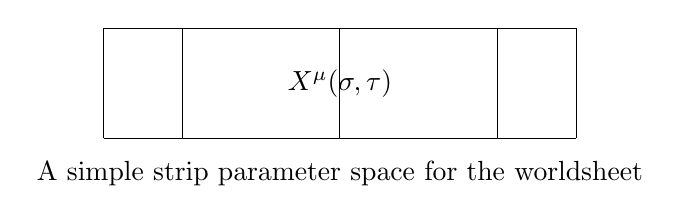
\begin{tikzpicture}[scale=1.0]
\draw (-3,0.7) -- (3,0.7);
\draw (-3,-0.7) -- (3,-0.7);
\draw (-3,-0.7) -- (-3,0.7);
\draw (3,-0.7) -- (3,0.7);
\draw (-2.0,-0.7) -- (-2.0,0.7);
\draw (0,-0.7) -- (0,0.7);
\draw (2.0,-0.7) -- (2.0,0.7);
\node at (0,0) {$X^\mu(\sigma,\tau)$};
\node at (0,-1.15) {A simple strip parameter space for the worldsheet};
\end{tikzpicture}
\caption{A clean redraw of the worldsheet strip labelled by the embedding field \(X^\mu(\sigma,\tau)\).}
\end{figure}

The important geometric move is that this one-boundary surface need not be described in only one way. By conformal mapping we may redraw the same worldsheet as a disk. That is not a change of physics. It is a change of coordinates, and for these equations that is exactly the freedom we have been preparing.

\subsection{Question \& Answer}

\paragraph{Question.} How do external momenta enter if the path integral integrates over all \(X^\mu\)?

\paragraph{Answer.} They do not enter through the bulk action alone. One must add extra factors associated with the external particles. Susskind pauses here and says that the strip picture is not the most convenient place to explain them. The disk picture is better, because the incoming and outgoing strings become boundary insertion points, and the momentum-carrying factors can be written directly there.

\section{Vertex Operators, Moduli, And The Electrostatics Reinterpretation}

On the disk, each external particle is represented by an insertion point on the boundary. For each such particle, with momentum \(k_i^\mu\), one includes a factor
\begin{equation}
e^{i k_i\cdot X(z_i)}=e^{i k_{i\mu}X^\mu(z_i)}.
\end{equation}
These are the vertex operators of the lecture. They are not the bulk action itself; they are the extra operators that inject momentum into the worldsheet.

\begin{figure}[h]
\centering

\includegraphics[width=0.72\textwidth]{lecture_08_figure_05.png}
\caption{Euclidean worldsheet weight and vertex insertions.}
\end{figure}

Thus the open-string tree amplitude takes the schematic form
\begin{equation}
\mathcal{A}_n \sim \int \mathcal{D}X \, e^{-S_E[X]} \prod_{i=1}^n e^{i k_i\cdot X(z_i)}.
\end{equation}
After performing the path integral over the embeddings, one still integrates over the positions \(z_i\) of the boundary insertions. The momenta \(k_i\) are fixed external data; it is the positions of their insertion that are integrated.

Because of conformal freedom, not all of those position integrals are independent. On the disk one may fix any three boundary points by a conformal transformation. Therefore, for \(n\) external open-string states, the number of remaining position integrals is
\begin{equation}
N_{\rm int}=n-3.
\end{equation}

\begin{figure}[h]
\centering
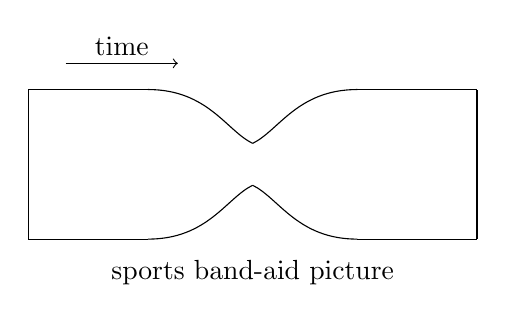
\begin{tikzpicture}[scale=0.95]
\draw (-3,1.0) -- (-1.4,1.0);
\draw (-1.4,1.0) .. controls (-0.6,1.0) and (-0.35,0.45) .. (0,0.28);
\draw (0,0.28) .. controls (0.35,0.45) and (0.6,1.0) .. (1.4,1.0);
\draw (1.4,1.0) -- (3,1.0);

\draw (-3,-1.0) -- (-1.4,-1.0);
\draw (-1.4,-1.0) .. controls (-0.6,-1.0) and (-0.35,-0.45) .. (0,-0.28);
\draw (0,-0.28) .. controls (0.35,-0.45) and (0.6,-1.0) .. (1.4,-1.0);
\draw (1.4,-1.0) -- (3,-1.0);

\draw (-3,-1.0) -- (-3,1.0);
\draw (3,-1.0) -- (3,1.0);
\draw[->] (-2.5,1.35) -- (-1.0,1.35);
\node at (-1.75,1.58) {time};
\node at (0,-1.45) {sports band-aid picture};
\end{tikzpicture}
\hspace{0.9cm}
\begin{tikzpicture}[scale=1.0]
\draw (0,0) circle (1.6);
\fill (1.6,0) circle (0.05);
\fill (0,1.6) circle (0.05);
\fill (-1.6,0) circle (0.05);
\fill (0,-1.6) circle (0.05);
\node at (1.95,0) {$z_1$};
\node at (0,1.95) {$z_2$};
\node at (-1.95,0) {$z_3$};
\node at (0,-1.95) {$z_4$};
\node at (0,-2.45) {disk picture};
\end{tikzpicture}
\caption{The same one-boundary worldsheet may be described either in a strip-like scattering picture or as a disk with boundary insertions.}
\end{figure}

Now comes the elegant final reinterpretation. Because the action is quadratic, the path integral is Gaussian. In the critical dimension one can carry it out, and the answer can be read as an electrostatics problem on the disk. Each field \(X^\mu\) behaves like an electrostatic potential. The components \(k_i^\mu\) of the external momenta behave like charges placed at the boundary insertion points. There are therefore \(26\) independent charge sectors in the bosonic theory, one for each \(\mu\).

The bulk field equations are again Laplace equations, now with sources supplied by the insertions. One solves the electrostatics problem, computes the electrostatic energy, adds the contributions from the distinct \(\mu\)-sectors, exponentiates minus that total energy, and then integrates over the allowed insertion positions. In that sense the whole amplitude becomes
\begin{equation}
\mathcal{A}_n \sim \int d(\hbox{boundary positions})\, e^{-E_{\rm electrostatic}}.
\end{equation}
The lecture does not stop to write a fully normalized energy functional, and it is better not to over-polish that point here. The conceptual point is already complete: string scattering has been converted into a Laplace problem with many kinds of boundary charge.

There is one more detail that Susskind answers explicitly. The \(i\) in \(e^{ik\cdot X}\) is the ordinary complex unit. It is not the \(i\) that was removed when \(\tau\) was Wick-rotated.

\subsection{Question \& Answer}

\paragraph{Question.} If this prescription is so simple, why is the physical theory not finished?

\paragraph{Answer.} Because the elegance of the formalism is not yet the realism of the theory. In the bosonic theory the path integral gives a sensible finite answer only in the critical dimension, namely \(26\). Outside that dimension one gets infinities. But \(26\)-dimensional bosonic string theory is obviously not a realistic description of the world we observe. One must compactify the extra dimensions, and that is where the real difficulty of the subject begins. The lecture is very explicit on this point: this is beautiful mathematics, but not yet a finished theory of elementary particles.

A related late remark in the lecture is that the external momenta \(k_i\) are not themselves quantized. They are continuous variables. What is quantized is the mass spectrum, that is, combinations built from sums of squares of momenta.

\section{Summary}

The lecture begins with two-dimensional electrostatics and ends by returning to it from an unexpected direction. In between, the key chain of ideas is tight: harmonic functions lead to analytic functions, analytic functions are conformal, conformal maps let us redraw worldsheets without changing the physics, and the resulting path integral for open-string scattering can be reinterpreted as an electrostatics problem on the disk.

That is the mathematical heart of this chapter. Conformal mapping is not an optional embellishment of the worldsheet formalism. It is the symmetry that makes the whole construction manageable. The final answer is beautifully simple in the critical dimension, but the lecture closes by insisting on a sober point: simplicity of prescription is not the same as physical completion, and the hard work lies beyond this first bosonic picture.